% !TEX root = ../notes_template.tex

\chapter{복소미분}

이 장에서는 다음 3가지 주제를 중점적으로 다룬다.

\begin{itemize}
\item[(1)] 복소미분의 정의:
즉, $\mathbb C$의 열린 부분집합 $U$에 정의된 함수 $f:U\to\mathbb C$와
$z_0\in U$가 주어졌을 때, ``$f$가 $z_0$에서 복소미분가능하고 복소미분값은 $f'(z_0)$이다''
라는 의미에 대하여 학습한다.
\item[(2)] 코시-리만 방정식: 
$\dfrac{\partial u}{\partial x} = \dfrac{\partial v}{\partial y}$와
$\dfrac{\partial u}{\partial y} = - \dfrac{\partial v}{\partial x}$.

이 방정식은 
복소미분가능함수 $f:U\to\mathbb C$의 실수부와 허수부 $u$, $v$가
만족하는 편미분방정식이다.

\begin{figure}[!h]
\begin{center}
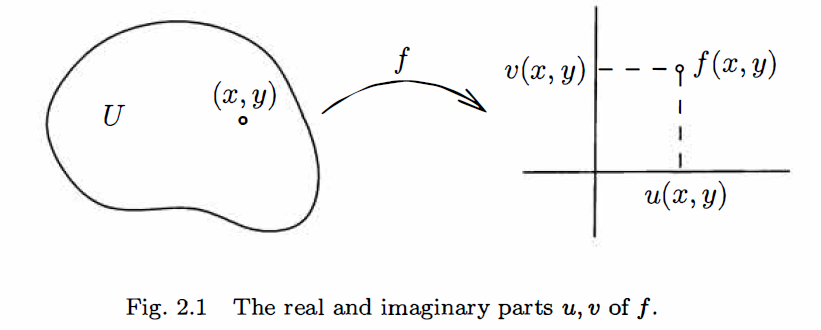
\includegraphics[width=0.6\textwidth]{./SaltChapter/fig-2-1}
\end{center}
\caption{$f$의 실수부와 허수부 $u$, $v$}
\label{fig-2-1}
\end{figure}

역으로, 어떤 열린집합 $U$의 모든 점에서 $C^1$-함수 $u, v$가 
코시-리만 방정식을 만족한다면 $f=u+iv$는 $U$에서 복소미분가능하다.

\item[(3)] 복소미분 $f'(z_0)$의 기하학적 의미:
국소적으로 보면, 함수 $f$는 $|f'(z_0)|$만큼 확대하면서
반시계방향으로 $\Arg(f'(z_0))$만큼 회전시키는 변환이다.
\end{itemize}

이 장에서는
열린집합에 정의된 복소미분가능함수가 
코시-리만 방정식을 만족할 필요충분조건(다소 덜 엄밀한 방식으로)에 대하여
중점적으로 다룬다.

\section{복소 미분가능성}

\begin{salt_definition}\label{def-2-1}
\
\begin{itemize}
\item[(1)] $U$가 $\mathbb C$의 열린 부분집합, $f: U\to \mathbb C$, $z_0\in U$라 하자.
다음 식을 만족하는 복소수 $L$이 존재하면, $f$가 $z_0$에서 {\bf 복소미분가능}이라 한다.
\[
\lim_{z\to z_0} \dfrac{f(z) - f(z_0)}{z - z_0} = L.
\]
즉, 임의의 $\epsilon>0$에 대하여 $\delta>0$가 존재하여,
$z\in U$, $0<|z-z_0|<\delta$이면 
\[
\left| \dfrac{f(z) - f(z_0)}{z - z_0} - L\right| < \epsilon
\]
을 만족한다.

극한값  $L$은 유일하게 결정되며 다음과 같이 나타낸다.
\[
f'(z_0) \quad\text{또는}\quad \dfrac{df}{dz}(z_0).
\]

\item[(2)] 열린집합 $U$에 정의된 함수 $f:U\to\mathbb C$가 $U$의 모든 점에서
복소미분가능하면 복소해석적(holomorphic\footnote{
``holomorphic''이라는 용어는 전체(entire)를 뜻하는 그리스어 ``holo''와
``모양(form)'' 또는 ``형세(apprearance)''을 나타내는 ``morphe''에서 파생되었다.
})이라 부른다.
\item[(3)] 복소수 $\mathbb C$ 전체에서 복소해석적이면 
전해석(entire) 함수라 부른다. 즉, $f$의 정의역이 복소수 $\mathbb C$ 전체이고
$\mathbb C$에서 복소해석적임을 의미한다.
\end{itemize}
\end{salt_definition}

전해석 함수의 간단한 예를 살펴보자.

\begin{salt_example} \label{example-2-1}
함수 $f:\mathbb C \to \mathbb C$를 $f(z) = z^2$ ($z\in\mathbb C$)라 정의하자.
그러면 $f$가 전해석 함수임을 보일 수 있다.
$z$가 $z_0$의 근방에 있을 때,
\[
\dfrac{f(z) - f(z_0)}{z - z_0} = \dfrac{z^2 - z_0^2}{z-z_0} = z + z_0 
\approx 2z_0
\]
이므로, $f'(z_0) = 2z_0$라고 추측할 수 있다.
이를 증명해 보자.
$z\ne z_0$에 대하여
\[
\left| \dfrac{f(z) - f(z_0)}{z - z_0} - 2z_0 \right|
= \left| \dfrac{z^2 - z_0^2}{z-z_0} - 2z_0 \right| 
= |z+z_0-2z_0| = |z-z_0|.
\]
따라서 $z$가 $z_0$에 충분히 가까우면
좌변을 원하는 만큼 작은 값으로 만들 수 있다.
$\epsilon>0$이라 하자.
$\delta:=\epsilon>0$으로 잡으면,
$z\in\mathbb C$가 $0<|z-z_0| <\delta$를 만족할 때마다
\[
\left| \dfrac{f(z) - f(z_0)}{z - z_0} - 2z_0 \right|
= |z-z_0| <\delta = \epsilon.
\]
결론적으로 $f'(z_0) = 2z_0$가 성립한다.
$z_0\in\mathbb C$를 임의로 선택할 수 있으므로,
$f$는 $\mathbb C$ 전체에서 복소해석적이고,
전해석 함수가 된다. 이상에서 다음 결론을 얻는다.
\[
\dfrac{d}{dz} z^2 = 2z, \quad z\in \mathbb C.
\]
\end{salt_example}

다른 방향으로, 이제 복소미분가능하지 않은 함수의 예를 보자.

\begin{salt_example} \label{example-2-2}
함수 $g:\mathbb C \to \mathbb C$를 $g(z) = \bar z$ ($z\in\mathbb C$)라 정의하자.
그러면 $g$는 어떤 점에서도 복소미분이 불가능함을 보일 수 있다.
$g$가 $z_0\in\mathbb C$에서 복소미분가능하다고 하자.
$\epsilon:=\frac12 >0$라 하면, $\delta>0$이 존재하여
$z$가 $0<|z-z_0|<\delta$를 만족할 때마다 
\[
\left| \dfrac{g(z)-g(z_0)}{z-z_0} - g'(z_0) \right| 
= \left| \dfrac{\bar z - \overline{z_0}}{z-z_0} - g'(z_0) \right| 
<\epsilon
\]
이 성립한다.

그림 \ref{fig-2-2}의 왼쪽을 보자.
위의 식에 따르면,
중심이 $z_0$이고 반지름이 $\delta$인 뚫린 원판(punctured disk)에 $z$가 속할 때마다
부등식이 성립함을 보장한다.
이제 그림의 뚫린 원판 내부에 $z_0$의 위쪽과 오른쪽에 한점씩을 선택하자.
이 점들을 부등식에 넣어보면, $g'(z_0)$는 각각 $-1$과 $1$을 중심으로 하고 반지름 $1/2$인
원판 내부에 속해야 한다.
그림 \ref{fig-2-2}의 오른쪽을 참고하면, 두 원판은 겹치치 않으므로 모순이 되어 증명이 끝난다.
아래에서 좀 더 자세히 살펴보자.

\begin{figure}[!h]
\begin{center}
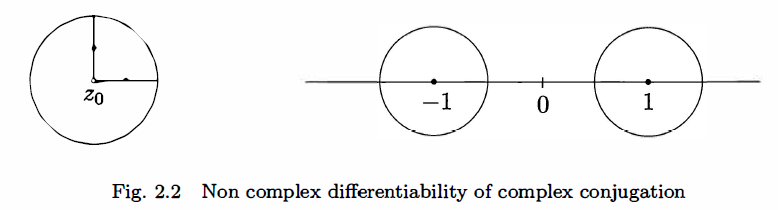
\includegraphics[width=0.8\textwidth]{./SaltChapter/fig-2-2}
\end{center}
\caption{켤레복소수 함수의 미분 불가능성}
\label{fig-2-2}
\end{figure}

$z=z_0+ \dfrac\delta2$로 잡으면, $0<|z-z_0|<\delta$이므로
\begin{equation} \label{eq-2-1}
\left| \dfrac{\bar z - \overline{z_0}}{z-z_0} - g'(z_0) \right| 
= \left| \dfrac{\delta/2}{\delta/2} - g'(z_0) \right| 
= | 1 - g'(z_0)| < \epsilon.
\end{equation}
한편, $z=z_0+ i\dfrac\delta2$로 잡으면, $0<|z-z_0|<\delta$이므로
\begin{equation} \label{eq-2-2}
\left| \dfrac{\bar z - \overline{z_0}}{z-z_0} - g'(z_0) \right| 
= \left| \dfrac{-\delta/2}{\delta/2} - g'(z_0) \right| 
= | 1 + g'(z_0)| < \epsilon.
\end{equation}
식 \eqref{eq-2-1}과 \eqref{eq-2-2}로부터
\[
2 = | 1- g'(z_0) + 1+ g'(z_0)|
\le |1-g'(z_0)| + |1+g'(z_0)| < \epsilon + \epsilon 
= 2\epsilon = 2\cdot\dfrac12 = 1
\]
이 되어 모순이다.
따라서 $g$는 $z_0$에서 복소미분가능하지 않다.
\end{salt_example}

\begin{salt_exercise} \label{ex-2-1}
모든 $z\in\mathbb C$에 대하여 $f(z) = |z|^2$로 정의된
함수 $f:\mathbb C \to \mathbb C$는 $0$에서 복소미분가능하며
$f'(0)=0$임을 보여라.
나중에 (연습문제 \ref{ex-2-9}에서) $f$는 $0$이 아닌 모든 점에서 복소미분 불가능함을 보일 것이다.
\end{salt_exercise}


\begin{salt_exercise} \label{ex-2-2}

\end{salt_exercise}

\begin{salt_exercise} \label{ex-2-3}

\end{salt_exercise}


\begin{salt_exercise} \label{ex-2-4}

\end{salt_exercise}


\begin{salt_exercise} \label{ex-2-5}

\end{salt_exercise}


\begin{salt_exercise} \label{ex-2-6}

\end{salt_exercise}


\begin{salt_exercise} \label{ex-2-7}

\end{salt_exercise}

\begin{salt_exercise} \label{ex-2-8}

\end{salt_exercise}

\begin{salt_exercise} \label{ex-2-9}

\end{salt_exercise}



